\documentclass[12pt, titlepage, oneside]{article}

\usepackage[margin=1in]{geometry}
\usepackage{siunitx, booktabs, amsmath, enumitem, pdfpages,mathrsfs,tabularx,caption, graphicx, pgfplots, textcomp,wrapfig, commath, svg, amsfonts, relsize}
\usepackage{parskip}
\usepackage[siunitx]{circuitikz}
\sisetup{detect-weight=true, detect-family=true}
\renewcommand{\vec}[1]{\oldvec{\bm{#1}}}
\renewcommand{\hat}[1]{\oldhat{\bm{#1}}}
\renewcommand{\b}[1]{\textbf{#1}}
\newcommand{\de}[1]{\noindent\fbox{\parbox{\textwidth}{#1}}}



\newcommand{\items}{\begin{itemize}}
\newcommand{\eitems}{\end{itemize}}


\newcommand{\ex}{Ex. }
\newcommand{\exe}{_}

\newcommand{\n}{\cap}
\renewcommand{\u}{\cup}


\begin{document}
	
	\textbf{ELECENG 3TQ3}\\
	\textbf{Elston A.}
	
\section{Lecture 4}
We can calculate the probability of the union between two sets in the following manner:
\begin{align*}
P[A\u B\u C] &= P[A] + P[B \u C] - P[A \n (B \u C)] \\
&= P[A] + P[B] + P[C] - P[A\u B] - P[A \u C] - P[B \u C] + P[A \u B \u C]
\end{align*}

\subsection{Magic Formula}

Since we know the probability of $P[A|B]$ is as follows
\begin{align*}
P[A|B] = \frac{P[A \n B]}{P[B]}
\end{align*}
so if we instead want the probability of B given A, that is $P[B|A]$ then we have the following formula
\begin{align*}
P[B|A] = \frac{P[A | B]P[B]}{P[A]}
\end{align*}
which we can replace the $P[A \n B]$ term in the numerator by $P[A|B] P[B]$
\begin{align}
P[B|A] = \frac{P[AB]}{P[A]} = \frac{P[A|B] P[B]}{P[A]}
\end{align}

\subsection{Consequences}

Total Probability of an event A when dealing with partitions is given as 
\begin{align}
	P[A] = \sum_{i=1}^m P[A|B_i]P[B_i]
\end{align}
so if we use Bayes theorem
\begin{align}
P[B_j | A] = \frac{P[A|B_j] P[B_j]}{\sum_{i=1}^m P[A|B_i]  P[B_i] }
\end{align}

\ex Consider tossing two different coins. Let C1 be the unfair tossing heads with a probability of 3/4 and let C2 be a fair coin tossing heads with probability 1/2. Lets assume that you randomly chose a coin and toss it. What is the probability that you selected C1 if you find out the coin toss was heads. 

In this case we would be looking for the probability we selected C1 given the outcome was H 
\begin{equation}
P[C1|H] = \frac{ P[H|C1]P[C1] }{P[H|C1]P[C1] + P[H|C2]P[C2]} = \frac{P[HC1]}{P[HC1] + P[HC2]} = \frac{3/8}{3/8+1/4} = \frac{3}{5}
\end{equation}


\subsection{Independent Events}

Two events are independent if and only if 
\begin{align}
P[AB] = P[A]P[B]
\end{align}
We should note that disjoint and independent are not the same. Mutually exclusive events mean they cannot happen at the same time, that is, if A and B are mutually exclusive then $P[AB] = 0$. 

Independent events are such events where observing one events does not change the outcome of the other. In other words, the conditional probability of an event does not change with the extra information about another event since they have no correlation.

Given two independent events A and B, 
\begin{align} 
P[A|B] = P[A] \enspace \enspace P[B|A] = P[B]
\end{align}

\ex Consider rolling two fair die. Let $A$ be the event that the product of the two numbers is 12, and let $B$ be the event the sum of the two numbers is 6. Are the events independent?

Since we know 6*2 = 2*6 = 4*3 = 3*4 = 12
\begin{align}
P[A] = \frac{4}{36}
\end{align}
Since we know 1+5 = 5+1 = 3+3 = 2+4 = 4+2 
\begin{align}
P[B] = 5/36
\end{align}
So we can see that $P[AB] = 0$ so these events are not independent, but disjoint

\subsection{Properties}
Let A and B be independent events, then A and $B^c$ are independent as well
\begin{align}
P[A\n B^c] = P[A] - P[A \n B] = P[A] - P[A]P[B]  = P[A](1-P[B]) = P[A]P[B^c]
\end{align}

\subsection{Three Events or More Events}
Consider 3 events A, B, C. They are independent if and only if
\items
\item A and B are independent
\item A and C are independent 
\item B and C are independent
\eitems

Thus we can say
\begin{align}
P[A \n B \n C] = P[ABC] = P[A]\n P[B]\n P[C] = P[A]P[B]P[C]
\end{align}
\b{Generalization}

For any $n$ events where $n \geq 3$ the sets $A_1,A_2,\dots,A_n$ where each set is independent from the other n-1 other sets.
\begin{align}
P[A_1 \n A_2 \n \dots \n A_n] = P[A_1]P[A_2]\dots P[A_n]
\end{align}
and in general
\begin{align}
P[A_1\u A_2 \u \dots \u A_n] = 1-P[A_1\n A_2 \n \dots \n A_n]
\end{align}

\ex Consider three independent events A, B, C and assume their probabilities are 0.5, 0.3, and 0.1. What is the probability that at least one event happens
\begin{align}
P[A\u B \u C] = 1- P[A]P[B]P[C] = 0.685
\end{align}
\subsection{Sequential Experiments}
Many experiments are done in stages where the next stage depends on the previous one. You can think of this as branches. 

As an example we have shown the sequential experiment of tossing a coin two times in a row.
\begin{figure}[h]
	\centering
	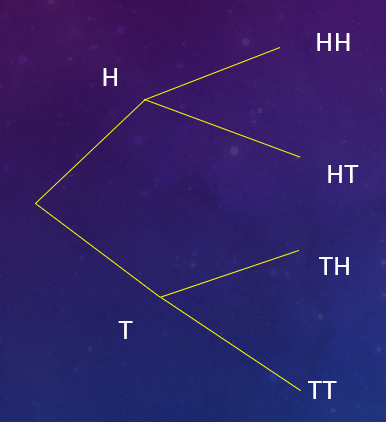
\includegraphics[width=0.5\linewidth]{images/toss}
	\caption{Coin toss outcomes}
	\label{fig:toss}
\end{figure}

Consider tossing a coin 5 times, recording the outcomes and repeating the whole process 10 times. We can define a success trial in many different ways. This type of method is often used in drug design and research. In these cases you perform n tests and record successes as 0 or 1. You can call a trial a success if a certain number of successes are recorded.



\end{document}
